\clearpage \documentclass[a4paper,12pt,notitlepage]{article}

\frenchspacing
\usepackage{a4}
\usepackage[pdftitle={Vypracovane otazky k bakalarskym statnicim}, pdfauthor={študenti MFF}, pdfdisplaydoctitle=true, colorlinks=false,unicode=true,pdfborder=0 0 0]{hyperref}
\usepackage{slovak}
\usepackage{ucs}
\usepackage[utf8x]{inputenc}

\title{Vypracovane otazky k bakalarskym statnicim}
\author{študenti MFF}

\usepackage{graphicx}
\usepackage{amsmath,amssymb,amsthm}
\usepackage{color}
\usepackage[left=3cm, right=3cm, top=3cm, bottom=3cm]{geometry} % nastavení dané velikosti okrajů


%Vacsina prostredi je dvojjazicne. V pripade, ze znenie napr pozorovania je pisane po slovensky, malo by byt po slovensky aj oznacenie.

\newenvironment{pozadavky}{\pagebreak[2]\noindent\textbf{Požadavky}\par\noindent\leftskip 10pt}{\par\bigskip}
\newenvironment{poziadavky}{\pagebreak[2]\noindent\textbf{Požiadavky}\par\noindent\leftskip 10pt}{\par\bigskip}

\newenvironment{definice}{\pagebreak[2]\noindent\textbf{Definice}\par\noindent\leftskip 10pt}{\par\bigskip}
\newenvironment{definiceN}[1]{\pagebreak[2]\noindent\textbf{Definice~}\emph{(#1)}\par\noindent\leftskip 10pt}{\par\bigskip}
\newenvironment{definicia}{\pagebreak[2]\noindent\textbf{Definícia}\par \noindent\leftskip 10pt}{\par\bigskip}
\newenvironment{definiciaN}[1]{\pagebreak[2]\noindent\textbf{Definícia~}\emph{(#1)}\par\noindent\leftskip 10pt}{\par\bigskip}

\newenvironment{pozorovani}{\pagebreak[2]\noindent\textbf{Pozorování}\par\noindent\leftskip 10pt}{\par\bigskip}
\newenvironment{pozorovanie}{\pagebreak[2]\noindent\textbf{Pozorovanie}\par\noindent\leftskip 10pt}{\par\bigskip}
\newenvironment{poznamka}{\pagebreak[2]\noindent\textbf{Poznámka}\par\noindent\leftskip 10pt}{\par\bigskip}
\newenvironment{poznamkaN}[1]{\pagebreak[2]\noindent\textbf{Poznámka~}\emph{(#1)}\par\noindent\leftskip 10pt}{\par\bigskip}
\newenvironment{lemma}{\pagebreak[2]\noindent\textbf{Lemma}\par\noindent\leftskip 10pt}{\par\bigskip}
\newenvironment{lemmaN}[1]{\pagebreak[2]\noindent\textbf{Lemma~}\emph{(#1)}\par\noindent\leftskip 10pt}{\par\bigskip}
\newenvironment{veta}{\pagebreak[2]\noindent\textbf{Věta}\par\noindent\leftskip 10pt}{\par\bigskip}
\newenvironment{vetaN}[1]{\pagebreak[2]\noindent\textbf{Věta~}\emph{(#1)}\par\noindent\leftskip 10pt}{\par\bigskip}
\newenvironment{vetaSK}{\pagebreak[2]\noindent\textbf{Veta}\par\noindent\leftskip 10pt}{\par\bigskip}
\newenvironment{vetaSKN}[1]{\pagebreak[2]\noindent\textbf{Veta~}\emph{(#1)}\par\noindent\leftskip 10pt}{\par\bigskip}

\newenvironment{dusledek}{\pagebreak[2]\noindent\textbf{Důsledek}\par\noindent\leftskip 10pt}{\par\bigskip}
\newenvironment{dosledok}{\pagebreak[2]\noindent\textbf{Dôsledok}\par\noindent\leftskip 10pt}{\par\bigskip}

\newenvironment{dokaz}{\pagebreak[2]\noindent\leftskip 10pt\textbf{Dôkaz}\par\noindent\leftskip 10pt}{\par\bigskip}
\newenvironment{dukaz}{\pagebreak[2]\noindent\leftskip 10pt\textbf{Důkaz}\par\noindent\leftskip 10pt}{\par\bigskip}

\newenvironment{priklad}{\pagebreak[2]\noindent\textbf{Příklad}\par\noindent\leftskip 10pt}{\par\bigskip}
\newenvironment{prikladSK}{\pagebreak[2]\noindent\textbf{Príklad}\par\noindent\leftskip 10pt}{\par\bigskip}
\newenvironment{priklady}{\pagebreak[2]\noindent\textbf{Příklady}\par\noindent\leftskip 10pt}{\par\bigskip}
\newenvironment{prikladySK}{\pagebreak[2]\noindent\textbf{Príklady}\par\noindent\leftskip 10pt}{\par\bigskip}

\newenvironment{algoritmusN}[1]{\pagebreak[2]\noindent\textbf{Algoritmus~}\emph{(#1)}\par\noindent\leftskip 10pt}{\par\bigskip}
%obecne prostredie, ktore ma vyuzitie pri specialnych odstavcoch ako (uloha, algoritmus...) aby nevzniklo dalsich x prostredi
\newenvironment{obecne}[1]{\pagebreak[2]\noindent\textbf{#1}\par\noindent\leftskip 10pt}{\par\bigskip}


\newenvironment{penumerate}{
\begin{enumerate}
  \setlength{\itemsep}{1pt}
  \setlength{\parskip}{0pt}
  \setlength{\parsep}{0pt}
  %\setlength{\topsep}{200pt}
  \setlength{\partopsep}{200pt}
}{\end{enumerate}}

\def\pismenka{\numberedlistdepth=2} %pouzit, ked clovek chce opismenkovany zoznam...

\newenvironment{pitemize}{
\begin{itemize}
  \setlength{\itemsep}{1pt}
  \setlength{\parskip}{0pt}
  \setlength{\parsep}{0pt}
}{\end{itemize}}

\definecolor{gris}{gray}{0.95}
\newcommand{\ramcek}[2]{\begin{center}\fcolorbox{white}{gris}{\parbox{#1}{#2}}\end{center}\par}
 \clearpage
\title{\LARGE Učební texty k státní bakalářské zkoušce \\ Programování \\ Programovací jazyky a překladače}
\begin{document}
\maketitle
\newpage
\setcounter{section}{3}
\section{Programovací jazyky a překladače}
\begin{pozadavky}
\begin{pitemize}
\item Principy a základy implementace objektově orientovaných jazyků a jazyků s blokovou strukturou, běhová podpora vyšších programovacích jazyků
\item Oddělený překlad, sestavení, řízení překladu
\item Neprocedurální programování
\item Struktura překladače, lexikální, syntaktická analýza
\item Interpretované jazyky, virtuální stroje
\item Pojmy a principy objektového návrhu
\item Generické programování a knihovny
\item Návrhové vzory
\end{pitemize}
\end{pozadavky}
\subsection{Principy a základy implementace objektově orientovaných jazyků a jazyků s blokovou strukturou, běhová podpora vyšších programovacích jazyků}

\textsl{Základní vědomosti:} \textit{ Třída, Dědičnost, Polymorfismus, Obalení, Virtuální funkce. Běhová podpora vyšších programovacích jazyků: Statická podpora a dynamická podpora, Rozdělení paměti, Stav paměti před spuštěním, Konstruktory, destruktory globálních proměnných, Volací konvence.}

TODO: jde hlavně o copy \& paste z Wikipedie, takže by to chtělo omezit zbytečné kecy a přeložit to, co je anglicky. Otázkou je taky, jestli sem úvodní článek vůbec patří. Ja myslím že jo, ale jistý si nejsem.

\subsubsection*{Strukturované programování}

Počítačový program je nějakým způsobem zaznamenaný postup počítačových operací, který speciálním způsobem popisuje praktickou realizaci zadané úlohy (tedy algoritmus výpočtu). Program z \emph{procedurálního} úhlu pohledu je vlastně přesná specifikace všech kroků, které musí počítač vykonat, aby došel k cíli, a jejich pořadí. Pro určování pořadí kroků se používají základní operace \emph{řízení toku} -- skoky, podmínky, cykly apod. 

Jedním z důležitých konceptů procedurálního programování je \emph{strukturované programování} -- jeho idea je založena na rodělení programu na \emph{procedury} (rutiny, podrutiny, metody, funkce), které samy obsahují výčet výpočetních kroků k vykonání, mohou být ale spouštěny opakovaně a z libovolného místa v programu. Jejich výhodou je mnohem názornější pohled na strukturu programu a snazší udržování kódu, než v případě použití jen nejjednoduššího řízení toku (tedy hlavně skoků, které by se ve strukturovaném programování správně používat neměly).

\medskip
Historically, several different structuring techniques or methodologies have been developed for writing structured programs. The most common are:
\begin{pitemize}
    \item \emph{Dijkstra's structured programming}, where the logic of a program is a structure composed of similar sub-structures in a limited number of ways. This reduces understanding a program to understanding each structure on its own, and in relation to that containing it, a useful separation of concerns.
    \item \emph{A view derived from Dijkstra's} which also advocates splitting programs into sub-sections with a single point of entry, but is strongly opposed to the concept of a single point of exit.
    \item \emph{Data Structured Programming}, which is based on aligning data structures with program structures. This approach applied the fundamental structures proposed by Dijkstra, but as constructs that used the high-level structure of a program to be modeled on the underlying data structures being processed. 
\end{pitemize}
The two latter meanings for the term "structured programming" are more common. Years after Dijkstra (1969), object-oriented programming (OOP) was developed to handle very large or complex programs.

\medskip
\begin{definiceN}{Programovací jazyk s blokovou strukturou}
A language is described as "block-structured" when it has a syntax for enclosing structures between bracketed keywords, such as an if-statement bracketed by \texttt{if..fi}, or a code section bracketed by \texttt{BEGIN..END}. 

However, a language is described as "comb-structured" when it has a syntax for enclosing structures within an ordered series of keywords. A "comb-structured" language has multiple structure keywords to define separate sections within a block, analogous to the multiple teeth or prongs in a comb separating sections of the comb. For example, in Ada, a block is a 4-pronged comb with keywords DECLARE, BEGIN, EXCEPTION, END, and the if-statement in Ada is a 4-pronged comb with keywords IF, THEN, ELSE, END IF. Jako jazyk s \uv{hřebenovou} strukturou by se dalo tedy brát třeba i PL/SQL.
\end{definiceN}

\begin{poznamka}
It is possible to do structured programming in any programming language, though it is preferable to use something like a procedural programming language. Since about 1970 when structured programming began to gain popularity as a technique, most new procedural programming languages have included features to encourage structured programming (and sometimes have left out features that would make unstructured programming easy). Some of the better known structured programming languages are Pascal, C, PL/I, and Ada.
\end{poznamka}

\begin{obecne}{Věta o strukturovaném programu???}
\emph{The structured program theorem} is a result in programming language theory. It states that every computable function can be implemented in a programming language that combines subprograms in only three specific ways. These three control structures are
\begin{pitemize}
    \item Executing one subprogram, and then another subprogram (\emph{sequence})
    \item Executing one of two subprograms according to the value of a boolean variable (\emph{selection})
    \item Executing a subprogram until a boolean variable is true (\emph{iteration})
\end{pitemize}

This observation did not originate with the structured programming movement; these structures are sufficient to describe the instruction cycle of a central processing unit, as well as the operation of a Turing machine. Therefore a processor is always executing a "structured program" in this sense, even if the instructions it reads from memory are not part of a structured program.
\end{obecne}


\subsubsection*{Datové a~řídící struktury vyšších programovacích jazyků a~jejich implementace}

\begin{obecne}{Řízení toku}
In computer science control flow (or alternatively, flow of control) refers to the order in which the individual statements, instructions or function calls of an imperative or functional program are executed or evaluated. Within an imperative programming language, a control flow statement is an instruction that when executed can cause a change in the subsequent control flow to differ from the natural sequential order in which the instructions are listed. For non-strict functional languages, functions and language constructs exist to achieve the same ends, but they are not necessarily called control flow statements.

The kinds of control flow statements available differ by language, but can be roughly categorized by their effect:
\begin{pitemize}
    \item continuation at a different statement (jump),
    \item executing a set of statements only if some condition is met (choice -- if-then-else)
    \item executing a set of statements zero or more times, until some condition is met (loop), s~podmínkou na začátku, na konci, uprostřed, nekonečné, s~daným počtem opakování
    \item executing a set of distant statements, after which the flow of control may possibly return (subroutines, coroutines, and continuations),
    \item stopping the program, preventing any further execution (halt).
\end{pitemize}
Interrupts and signals are low-level mechanisms that can alter the flow of control in a way similar to a subroutine, but are usually in response to some external stimulus or event rather than a control flow statement in the language. 
\end{obecne}

\begin{obecne}{Výjimky}
Výjimky jsou speciálním příkazem řízení toku, vyskytujícím se v některých vyšších programovacích jazycích. Základní myšlenkou je, že program může na nějakém místě vyhodit výjimku (příkaz \texttt{throw}), což způsobí, že provádění programu se zastaví a buď pokračuje tam, kde je výjimka \uv{ošetřena} (tzv. \texttt{catch} blok), nebo pokud takové místo není nalezeno, program skončí s chybou. Během hledání místa ošetření je datová hodnota výjimky uložena stranou a pak může být použita.

Při hledání místa ošetření výjimky (\texttt{try}-bloku, následovaného catch-blokem se správným datovým typem výjimky) se postupuje zpět po zásobníku volání funkcí, tato technika se nazývá \uv{stack unwinding} (odvíjení zásobníku). V některých jazycích (Java) lze definovat i akci, která se provede v každém případě, i pokud nastane výjimka, ještě před odvíjením zásobníku -- \texttt{finally} blok.
\end{obecne}

\begin{obecne}{Volací konvence}
Při volání procedur a funkcí je nejdůležitější zásobník. Ukládá se na něj
\begin{pitemize}
    \item kam se vrátit po volání
    \item argumenty funkce (v překladem definovaném pořadí -- nutné mít ve všech modulech stejné; většinou se liší v závislosti na programovacím jazyku)
    \item návratová hodnota funkce
    \item ukazatel na sémanticky nadřazenou funkci (Pascal) 
\end{pitemize}
Dohromady všem těmto datům se někdy říká \uv{aktivační záznam} procedury. Po skončení funkce je nutné zásobník opět uklidit (vymazat zbytečná uložená data, většinou jen zůstává návratová hodnota) a která část programu to dělá (volaná nebo volající procedura), závisí opět na překladači a konvenci jazyka.

\medskip\noindent
Volací konvence dvou nejtypičtějších jazyků:
\begin{pitemize}
	\item \emph{Pascal} \\ uklízí volaná funkce, argumenty se ukládají na zásobník zleva doprava (nejlevejší nejdřív, tj. nejhlouběji)
	\item \emph{C} \\ uklízí funkce volající, argumenty se ukládají zprava doleva (tj. nejlevější je na vrcholu zásobníku. Je to kvůli funkcím s proměnným počtem parametrů. Volaná funkce musí podle prvního argumentu poznat, jaký je skutečný počet argumentů. Kdyby byl první argument někde hluboko v~zásobníku, tak ví prd.)
\end{pitemize}
\end{obecne}


\subsubsection*{Organizace paměti}

Paměť procesu (spuštěného programu) lze rozdělit do několika částí:
\begin{pitemize}
	\item \emph{kód programu (kódový segment)} \\
vytvořen při překladu, součást spustitelného souboru, neměnný a má pevnou délku; obvykle bývá chráněn proti zápisu
	\item \emph{statická data (datový segment)} \\
data programu, jejichž velikost je známa již při překladu a jejichž pozice se během programu nemění (je připraven kompilátorem a jeho formát je taktéž zadrátovaný ve spustitelném souboru, u inicializovaných statických dat je tam celý uložený); v jazyce C jde o globální proměnné a lokální data deklarovaná jako \texttt{static}, konstanty
	\item \emph{halda (heap segment)} \\
vytvářen startovacím modulem (C Runtime library), ukládají se sem dynamicky vznikající objekty (\texttt{malloc, new}) -- neinicializovaná data, i seznam volného místa
	\item \emph{volná paměť} \\
postupně jí zaplňuje z jedné strany zásobník a z druhé halda
	\item \emph{zásobník (stack segment)} \\ 
informace o volání procedur (\uv{aktivační záznamy}) --- návratové adresy, parametry a návratové hodnoty (nejsou-li předávány v registrech), některé jazyky (Pascal, C) používají i pro úschovu lokálních dat. Typicky roste zásobník proti haldě (od \uv{konce} paměti k nižším adresám). 
\end{pitemize}


\begin{poznamkaN}{Vnořené funkce}
V Pascalu mohou být funkce definované uvnitř jiné funkce. Ta vnitřní potřebuje přistupovat k~proměnným té vnější. Proměnné jsou sice na zásobníku, ale pouhý odkaz na volající funkci nestačí, protože se vnořená funkce může volat rekurzivně. Proto je na zásobníku ukazatel na funkci sémanticky nadřazenou.
\end{poznamkaN}

\begin{obecne}{Alokace místa pro různé typy proměnných}
\begin{pitemize}
    \item Dynamicky alokované proměnné (přes pointer) se alokují na haldě. Opakovanou alokací a~dealokací paměťových bloků různé velikosti vznikají v~haldě \uv{díry} (střídavé úseky volného a naalokovaného místa). Existuje několik strategií pro vyhledání volného bloku požadované velikosti (first-fit, next-fit, buddy systém) a udržení informací o volném místě, které jsou většinou implementovány v knihovních funkcích jazyka (C, Pascal).
    \item Lokální proměnné se ukládají na zásobník, po skončení funkce, které přísluší, jsou zase odstraněny.
    \item Globální a~statické se ukládají do segmentu pro statická data. Tady se díry tvořit nebudou, protože tyhle proměnné vznikají na začátku a~zanikají na konci programu (takže se formát segmentu nemění).
\end{pitemize}
\end{obecne}



\subsubsection*{Objektově-orientované programování}

\begin{obecne}{Účel objektového porgramování}
In the 1960s, language design was often based on textbook examples of programs, which were generally small (due to the size of a textbook); however, when programs become very large, the focus changes. In small programs, the most common statement is generally the assignment statement; however, in large programs (over 10,000 lines), the most common statement is typically the procedure-call to a subprogram. Ensuring parameters are correctly passed to the correct subprogram becomes a major issue.

Many small programs can be handled by coding a hierarchy of structures; however, in large programs, the organization is more a network of structures, and insistence on hierarchical structuring for data and procedures can produce cumbersome code with large amounts of "tramp data" to handle various options across the entire program. 

Although structuring a program into a hierarchy might help to clarify some times of software, even for some special types of large programs, a small change, such as requesting a user-chosen new option (text font-color) could cause a massive ripple-effect with changing multiple subprograms to propagate the new data into the program's hierarchy. The object-oriented approach is allegedly more flexible, by separating a program into a network of subsystems, with each controlling their own data, algorithms, or devices across the entire program, but only accessible by first specifying named access to the subsystem object-class, not just by accidentally coding a similar global variable name. Rather than relying on a structured-programming hierarchy chart, object-oriented programming needs a call-reference index to trace which subsystems or classes are accessed from other locations.
\end{obecne}


\begin{definiceN}{Objektově orientované programování}
Na objektově-orientované programování se dá nahlédnout jako na kolekci spolupracujících objektů -- v protikladu k tradičnímu pohledu, kdy se za program považuje sled instrukcí pro počítač. V OOP je každý objekt schopný přijímat zprávy, zpracovávat data a posílat zprávy jiným objektům. Na každý objekt se tak dá nahlížet jako na nezávislý \uv{malý stroj} s vlastní rolí a zodpovědností. Zjednodušeně řečeno jde o~dotažení konceptu \emph{data + algoritmy = program}. Data tvoří s kódem, který je spravuje, jeden celek.
\end{definiceN}

\begin{obecne}{Hlavní koncepty (a formálnější definice)}
Objektově orientované programování (zkracováno na OOP, z anglického Object-oriented programming) je metodika vývoje softwaru, založená na následujících myšlenkách, koncepci:
\begin{pitemize}
	\item \emph{Objekty}: jednotlivé prvky modelované reality (jak data, tak související funkčnost) jsou v programu seskupeny do entit, nazývaných objekty. Objekty si pamatují svůj stav a navenek poskytují operace (přístupné jako metody pro volání).
	\item \emph{Abstrakce}: programátor, potažmo program, který vytváří, může abstrahovat od některých detailů práce jednotlivých objektů. Každý objekt pracuje jako černá skříňka, která dokáže provádět určené činnosti a komunikovat s okolím, aniž by vyžadovala znalost způsobu, kterým vnitřně pracuje.
	\item \emph{Zapouzdření}: zaručuje, že objekt nemůže přímo přistupovat k \uv{vnitřnostem} jiných objektů, což by mohlo vést k nekonzistenci. Každý objekt navenek zpřístupňuje rozhraní, pomocí kterého (a nijak jinak) se s objektem pracuje.
	\item \emph{Skládání}: Objekt může využívat služeb jiných objektů tak, že je požádá o provedení operace.
	\item \emph{Dědičnost}: objekty jsou organizovány stromovým způsobem, kdy objekty nějakého druhu mohou dědit z jiného druhu objektů, čímž přebírají jejich schopnosti, ke kterým pouze přidávají svoje vlastní rozšíření. Tato myšlenka se obvykle implementuje pomocí rozdělení objektů do tříd, přičemž každý objekt je instancí nějaké třídy. Každá třída pak může dědit od jiné třídy (v některých programovacích jazycích i z několika jiných tříd). Umožňuje zacházet s~množinou tříd, jako by byly všechny reprezentovány tím samým objektem. Například známá hierarchie: grafický objekt, bod, kružnice. Navíc je to prostředek pro úsporu práce při kódování.
	\item \emph{Polymorfismus}: odkazovaný objekt se chová podle toho, jaký je jeho skutečný typ. Pokud několik objektů poskytuje stejné rozhraní, pracuje se s nimi stejným způsobem, ale jejich konkrétní chování se liší. V praxi se tato vlastnost projevuje např. tak, že na místo, kde je očekávána instance nějaké třídy, můžeme dosadit i instanci libovolné její podtřídy (třídy, která přímo či nepřímo z této třídy dědí), která se může chovat jinak, než by se chovala instance rodičovské třídy, ovšem v rámci \uv{mantinelů}, daných popisem rozhraní. 
\end{pitemize}
\end{obecne}

\begin{obecne}{Třída}
\emph{Třída} definuje abstraktní vlastnosti nějakého objektu, vřátaně obsáhnutých dat (atributy, pole (fields) a vlastnosti (properties)) a věcí, které může dělat (správaní, metody a schopnosti (features)). Například třída \emph{Dog} by obsahovala věci spoločné pro všechny psy - např. atribúty rasa, barba srsti a schopnosti břechat. % tady prosim ten jazyk neopravujte, to je tak hezky :)!
 

Třídy poskytují v objektovo-orientovaném programu modularitu a strukturu. Třída by typicky měla být rozpoznatelná i ne-programátorovi, který se ale v dané doméně problémů orientuje -- tzn. že charakteristiky třídy by měli \uv{dávat v kontextu smysl}. Podobně i kód třídy by měl být relativně \uv{self-contained}. Vlastnosti a metódy tříd se spolu nazývají i \emph{members}.
\end{obecne}

\begin{obecne}{Implementace objektů}
Z hlediska jazyka není velký rozdíl mezi složenými datovými typy a třídami. Deklarace třídy obsahuje, stejně jako u složeného dat. typu, datové položky. Navíc ale obsahuje i deklarace funkcí (metod), které s nimi pracují. Některé funkce mohou mít speciální vlastnosti -- statické, virtuální, konstruktory, destruktory. Navíc většina jazyků přidává možnost označení kterýchkoliv položek jako veřejné nebo privátní. Třídy mohou někdy (C++, Java) obsahovat i vnořené datové typy (výčty, ... ) a dokonce vnořené třídy.

Za běhu je jedna instance třídy -- objekt reprezentována v paměti pomocí:
\begin{pitemize}
    \item datových položek (stejně jako složený datový typ),
    \item skrytých pomocné položky umožňujících funkci virtuálních metod, výjimek, RTTI a dědičnosti (identifikace typu / jeho velikosti apod.)
\end{pitemize}

\emph{Implementace dědičnosti v C++:} Je-li třída B (přímým či nepřímým) potomkem třídy A, pak paměťová reprezentace objektu typu B obsahuje část, která má stejný tvar jako paměťová reprezentace samostatného objektu typu A. Z každého ukazatele na typ B je možno odvodit ukazatel na část typu A -- tato konverze je implicitní, tj. není třeba ji explicitně uvádět ve zdrojovém kódu. Tato konverze může (obvykle pouze při násobné dědičnosti) vyžadovat jednoduchý výpočet (přičtení posunutí).

Z ukazatele na typ A je možno odvodit ukazatel na typ B, jen pokud konkrétní objekt, do kterého ukazuje ukazatel na typ A, je typu B (nebo jeho potomka). Zodpovědnost za ověření skutečného typu objektu má programátor a tuto konverzi je třeba explicitně vynutit přetypováním. Může to znamenat odečtení posunutí v paměti.
\end{obecne}

\begin{obecne}{Virtuální funkce}
In object-oriented programming (OOP), a virtual function or virtual method is a function whose behavior, by virtue of being declared "virtual," is determined by the definition of a function with the same signature furthest in the inheritance lineage of the instantiated object on which it is called. This concept is a very important part of the polymorphism portion of object-oriented programming (OOP).

The concept of the virtual function solves the following problem:

In OOP when a derived class inherits from a base class, an object of the derived class may be referred to (or cast) as either being the base class type or the derived class type. If there are base class functions overridden by the derived class, a problem then arises when a derived object has been cast as the base class type. When a derived object is referred to as being of the base's type, the desired function call behavior is ambiguous.

The distinction between virtual and not virtual is provided to solve this issue. If the function in question is designated "virtual" then the derived class's function would be called (if it exists). If it is not virtual, the base class's function would be called.

\emph{Pozdní vazba (late binding; virtual call):} Je-li metoda nějaké třídy virtuální či čistě virtuální, pak všechny metody se stejným jménem, počtem a typy parametrů deklarované v potomcích třídy jsou považovány za různé implementace téže funkce. Která implementace se vybere, tedy které tělo bude zavoláno, se rozhoduje až za běhu programu podle skutečného typu celého objektu. Použije se tělo z posledního potomka, který definuje tuto funkci a je součástí celého objektu. Pozdní vazba má smysl pouze u vyvolání na objektu určeném odkazem.

Pozdní vazba je implementačně umožněná skrytým pointerem na \emph{tabulku virtuálních funkcí} uvnitř každého objektu. Existuje pro každou třídu jedna. Při dědičnosti zůstává v celém objektu odkaz jeden, ale (i pro \uv{nejvnitřnější} bázovou třídu) odkazuje na tabulku odvozené třídy. V tabulce musí být proto pointery na funkce, deklarované už u bázové třídy, umístěny na začátku (aby bylo možné volat funkce bázové třídy mezi sebou bez změny kódu).
\end{obecne}


\subsection{Oddělený překlad, sestavení, řízení překladu}

\subsubsection*{Struktura programu}

Program se skládá z \emph{modulů}:
\begin{pitemize}
	\item Překládány samostatně kompilátorem 
	\item Spojovány linkerem
\end{pitemize}
Modul z pohledu programátora
\begin{pitemize}
	\item Soubor s příponou .cpp (.c)
\end{pitemize}
Hlavičkové soubory
\begin{pitemize}
	\item Soubory s příponou .h
	\item Deklarují (a někdy i definují) identifikátory používané ve více modulech
	\item Vkládány do modulů direktivou include
	\begin{pitemize}
		\item Direktivu zpracovává preprocesor čistě textově
		\item Preprocesor je integrován v kompilátoru jako první fáze překladu
	\end{pitemize}
\end{pitemize}
Modul z pohledu kompilátoru
\begin{pitemize}
	\item Samostatná jednotka překladu
	\item Výsledek práce preprocesoru
\end{pitemize}

\subsubsection*{Oddělený překlad}

\par\begin{center}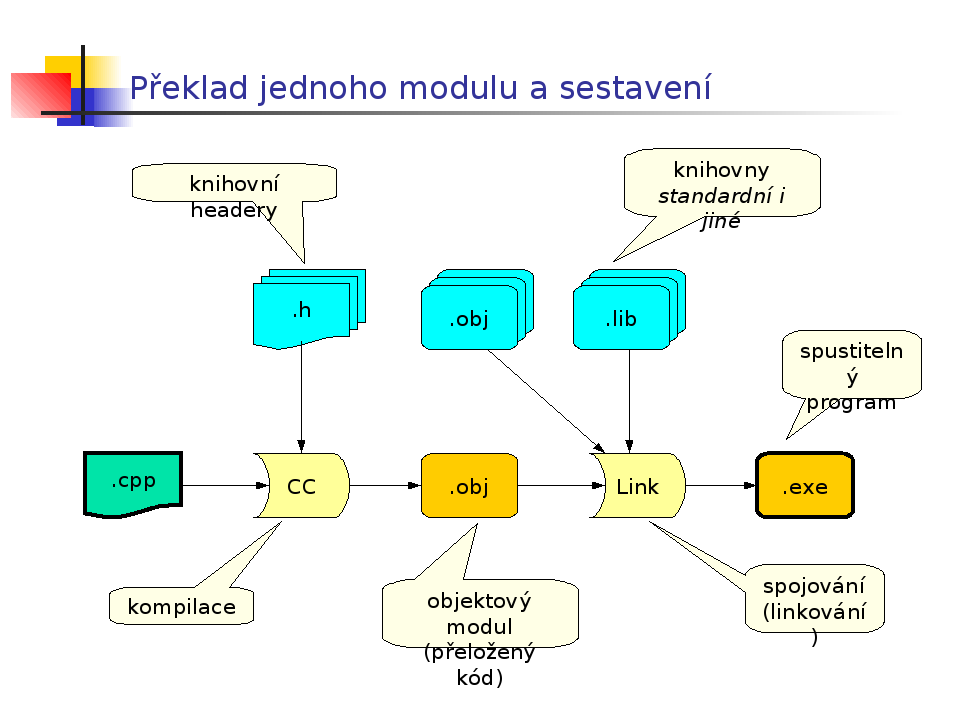
\includegraphics[width=10cm]{informatika/programovanie/obrazky/oddelenypreklad01.png}
\end{center}
\par\begin{center}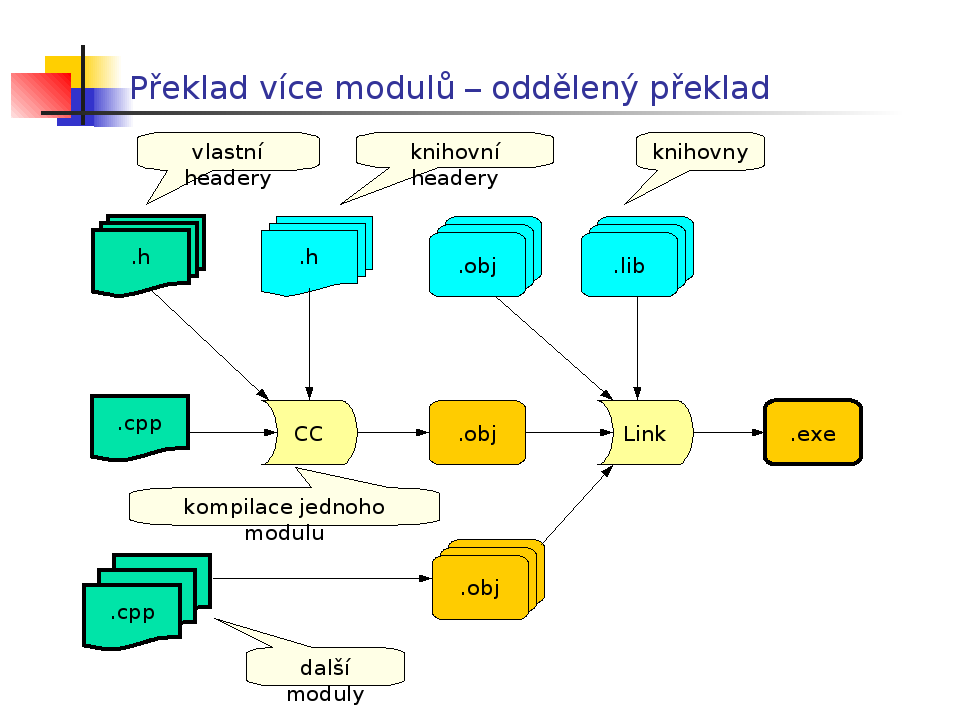
\includegraphics[width=10cm]{informatika/programovanie/obrazky/oddelenypreklad02.png}\end{center}
Smysl odděleného překladu modulů je urychlení celkového překladu -- nepřekládat to, co se od minula nezměnilo. Oddělený překlad dnes díky automatizaci makefily (viz níže) a integrovanými prostředími není téměř pro programátora vidět.

...pri tomto slide je vhodné ujasniť si, ako funguje statické a dynamické linkovanie (ako, kde a kedy sa opravujú adresy objektov atď.):
\begin{pitemize}
    \item \emph{Statické linkování} \\ Po odděleném překladu jednotlivé object moduly ještě neobsahují přímo adresy všech funkcí a externích identifikátorů, jen odkazy na ně. Linker se postará o jejich spojení dohromady. Je nutné, aby jména byla unikátní, takže u přetížených a virtuálních funkcí, jako je v C++, musí bý jména zpotvořena tak, aby ukazovala i třídu, namespace, parametry a jejich typy. To má na starosti compiler a říká se tomu \emph{name mangling}.
    \item \emph{Dynamické linkování} \\ Nastává po volání operačního systému -- zavedení dynamické knihovny do paměti. Jsou dvě možnosti jeho provedení, první je právě při zavádění knihovny, kdy se odkazy na všechny funkce (a mezi nimi navzájem) naplní správnými hodnotami (podle bázové adresy, na kterou se knihovna do paměti nahraje). Druhá možnost je použití dvou pointerů při volání funkcí z knihovny -- to se vytvoří tabulka skutečných adres, na kterou se z knihovny ukazuje. První možnost trvá déle při zavádění knihovny, druhá je zase pomalejší při provádění, ale umožňuje kód knihovny beze změn sdílet více procesy.
\end{pitemize}


\par\begin{center}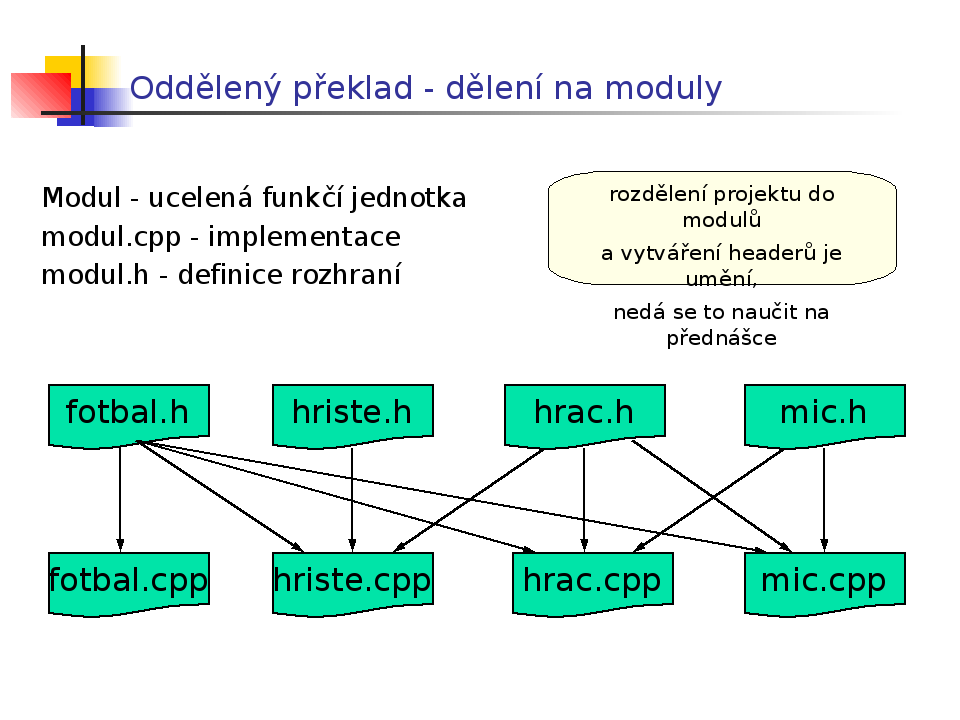
\includegraphics[width=10cm]{informatika/programovanie/obrazky/oddelenypreklad03.png}\end{center}

\emph{Linker} je program, který prijímá jeden alebo více objektů generovaných kompilátorem a složí je v jeden spustitelný program.

Objektový kód, nebo objektový soubor je reprezentace kódu, který kompilátor nebo assembler vytvoří zpracováním zdrojového kódu. Objektové soubory obsahují kompaktní kód, často nazývaný \uv{binárky} :-) Linker se typicky používá na vytvoření spustitelnýho souboru nebo knihovny spojením (slinkováním) objektových souborů. Základní častí objektového souboru je strojový kód (kód přimo vykonávaný CPU počítače).

\subsubsection*{Makefile}

Smyslem programu \emph{make} je řízení překladu a linkování. Popis závislostí jednotlivých modulů a hlavičkových na sobě je definován v 1 textovém souboru -- \emph{Makefile} (tj. které soubory je nutné mít aktuální/vytvořené pro překlad kterého souboru). Make vždy po změně souboru přeloží jen to, co na něm závisí.
Formát souboru make:
\begin{verbatim}
targets: files; 
        commands; #comment; line-begin\
        line contd.;
\end{verbatim}
Targets -- cíle činností / cílové soubory, možno definovat vic, při spuštění make bez parametrů se bere první; univ. nástroj (nejen pro překlad C/C++). Lze definovat i vlastní makra (příkazem \texttt{<název makra> = <string>}) a pak je používat (\texttt{\$\{makro\}}).

\subsection{Neprocedurální programování, logické programování}

\subsubsection*{Neprocedurální programování}
\emph{Deklarativní programování} je postaveno na paradigmatu, podle něhož je program založen na tom, co se počítá a ne jak se to počítá. Je zde deklarován vstup a výstup a celý program je chápán jako funkce vyhodnocující vstupy podávající jediný výstup. Například i webovské stránky jsou deklarativní protože popisují, jak by stránka měla vypadat -- titulek, font, text a obrázky -- ale nepopisují, jak konkrétně zobrazit stránky na obrazovce.

\emph{Logické programování} a \emph{funkcionální programování} jsou poddruhy deklarativního programování. Logické programování využívá programování založené na vyhodnocování vzorů - tvrzení a cílů. Klasickým zástupcem jazyka pro podporu tohoto stylu je Prolog.

Tento přístup patří pod deklarativní programování stejně jako funkcionální programování, neboť deklaruje, co je vstupem a co výstupem, a nezabývá se jak výpočet probíhá. Naopak program jako posloupnost příkazů je paradigma imperativní.

\emph{Funkcionální programování} patří mezi deklarativní programovací principy.

Alonzo Church vytvořil formální výpočtový model nazvaný $\lambda$-kalkul. Tento model slouží jako základ pro funkcionální jazyky. Funkcionální jazyky dělíme na:
\begin{pitemize}
	\item typované - Haskell
	\item netypované - Lisp, Scheme
\end{pitemize}

Výpočtem funkcionálního programu je posloupnost vzájemně ekvivalentních výrazů, které se postupně zjednodušují. Výsledkem výpočtu je výraz v normální formě, tedy dále nezjednodušitelný. Program je chápán jako jedna funkce obsahující vstupní parametry mající jediný výstup. Tato funkce pak může být dále rozložitelná na podfunkce.

\subsubsection*{Prolog}

Prolog je logický programovací jazyk. Název Prolog pochází z francouzského programmation en logique (\uv{logické programování}). Byl vytvořen Alainem Colmerauerem v roce 1972 jako pokus vytvořit programovací jazyk, který by umožňoval vyjadřování v logice místo psaní počítačových instrukcí. Prolog patří mezi tzv. deklarativní programovací jazyky, ve kterých programátor popisuje pouze cíl výpočtu, přičemž přesný postup, jakým se k výsledku program dostane, je ponechán na libovůli systému.

Prolog je využíván především v oboru umělé inteligence a v počítačové lingvistice (obzvláště zpracování přirozeného jazyka, pro nějž byl původně navržen). Syntaxe jazyka je velice jednoduchá a snadno použitelná pravě proto, že byl původně určen pro počítačově nepříliš gramotné lingvisty.

Prolog je založen na \emph{predikátové logice prvního řádu} (konkrétně se omezuje na Hornovy klauzule). Běh programu je pak představován aplikací dokazovacích technik na zadané klauzule. Základními využívanými přístupy jsou \emph{unifikace}, \emph{rekurze} a \emph{backtracking}.

Interpret Prologu se snaží nalézt nejobecnější substituci, která splní daný cíl - tzn. nesubstituuje zbytečně, pokud nemusí (použití interních proměnných -- \_123 atd.). Za dvě proměnné může být substituována jedna interní proměnná (např. při hledání svislé úsečky -- konstantní X souřadnice) -- tomu se říká \emph{unifikace} proměnných. Pro proměnnou, jejíž hodnota může být libovolná, se v prologu užívá znak \uv{\_}. 

Datové typy v prologu se nazývají \emph{termy}. Základním datovým typem jsou \emph{atomy} (začínají malým písmenem, nebo se skládají ze speciálních znaků (\texttt{+ - * / \dots}, nebo jsou to znakové řetězce (\texttt{'text'})). Dále \uv{jsou} v prologu čísla (v komerčních implementacích i reálná), proměnné (velké písmeno) a struktury (definované rekursivně - pomocí funktoru dané arity a příslušným počtem termů, které jsou jeho argumenty -- \texttt{okamzik(datum(1,1,1999),cas(10,10))}). Posledním typem proměnných jsou seznamy, které jsou probírány později.

\medskip\textbf{Základní principy}:

Programování v Prologu se výrazně liší od programování v běžných procedurálních jazycích jako např. C. Program v prologu je databáze faktů a pravidel (dohromady se faktům a pravidlům paradoxně říká procedury), nad kterými je možno klást dotazy formou tvrzení, u kterých Prolog zhodnocuje jejich pravdivost (dokazatelnost z údajů obsažených v databázi).

Například lze do databáze uložit fakt, že Monika je dívka:
\begin{verbatim}
dívka(monika).
\end{verbatim}

Poté lze dokazatelnost tohoto faktu prověřit otázkou, na kterou Prolog odpoví yes (ano):
\begin{verbatim}
?- dívka(monika).
     yes.
\end{verbatim}

Také se lze zeptat na všechny objekty, o kterých je známo, že jsou dívky (středníkem požadujeme další výsledky):
\begin{verbatim}
?- dívka(X).
     X = monika;
     no.
\end{verbatim}

Pravidla (závislosti) se zapisují pomocí implikací, např.
\begin{verbatim}
syn(A,B) :- rodič(B,A), muž(A).
\end{verbatim}

Tedy: pokud B je rodičem A a zároveň je A muž, pak A je synem B. První části pravidla (tj. důsledku) se říká hlava a všemu co následuje za symbolem \texttt{:-} (tedy podmínkám, nutným pro splnění hlavy) se říká tělo. Podmínky ke splnění mohou být odděleny buď čárkou (pak jde o konjunkci, musejí být splněny všechny), nebo středníkem (disjunkce), přičemž čárky mají větší prioritu.

\medskip\textbf{Příklad}:

Typickou ukázkou základů programování v Prologu jsou rodinné vztahy.
\begin{verbatim}
sourozenec(X,Y) :- rodič(Z,X), rodič(Z,Y).
rodič(X,Y) :- otec(X,Y).
rodič(X,Y) :- matka(X,Y).
muž(X) :- otec(X,_).
žena(X) :- matka(X,_).
matka(marie,monika).
otec(jiří,monika).
otec(jiří,marek).
otec(michal,tomáš).
\end{verbatim}

Prázdný seznam je označen atomem $[]$, neprázdný se tvoří pomocí funktoru \texttt{'.'} (tečka) - \texttt{.(Hlava,Tělo)}. V praxi se to (naštěstí ;-)) takhle složitě rekurzivně zapisovat nemusí, stačí napsat \texttt{[a,b,c...]}, resp \texttt{[Začátek | Tělo]}, kde začátek je výčet prvků (ne seznam) stojících na začátku definovaného seznamu, a tělo je (rekurzivně) seznam (např. \texttt{[a,b,c|[]]}).

Aritmetické výrazy se samy o sobě nevyhodnocují, dokud jim to někdo nepřikáže. Takže např. predikát \texttt{5*1 = 5} by selhal. Vyhodnocení se vynucuje pomocí operátoru \emph{is} (pomocí = by došlo jen k unifikaci) - není to ale ekvivalent \uv{\texttt{=}} z jiných jazyků. Tento operátor se musí použít na nějakou volnou proměnnou a aritmetický výraz, s jehož hodnotou bude tato proměnná dále svázaná (jako např. \texttt{X is 5*1,X=5} uspěje).

Důležitý je i \emph{operátor řezu} (značíme vykřičníkem). Tento predikát okamžitě uspěje, ale při tom zakáže backtrackování přes sebe zpět. (\texttt{prvek1(X,[X|L]):-!. prvek1(X,[\_|L]):-prvek1(X,L).} - je-li prvek nalezen, je zakázán návrat = najde jen první výskyt prvku). Dále je důležitá negace (\texttt{not(P):- P, !, fail. not(P).} -- uspěje, pokud se nepodaří cíl P splnit). Řez tedy umožňuje ovlivňovat efektivitu prologovských programů, definovat vzájemně se vylučující použití jednotlivých klauzulí procedury, definovat negaci atd.

\subsubsection*{Haskell}
Haskell je standardizovaný funkcionální programovací jazyk používající zkrácené vyhodnocování, pojmenovaný na počest logika Haskella Curryho. Byl vytvořen v 80. letech 20. století. Posledním polooficiálním standardem je Haskell 98, který definuje minimální a přenositelnou verzi jazyka využitelnou k výuce nebo jako základ dalších rozšíření. Jazyk se rychle vyvíjí, především díky svým implementacím Hugs a GHC (viz níže).

Haskell je jazyk dodržující \emph{referenční transparentnost}. To, zjednodušeně řečeno, znamená, že tentýž (pod)výraz má na jakémkoliv místě v programu stejnou hodnotu. Mezi další výhody tohoto jazyka patří přísné \emph{typování proměnných}, které programátorovi může usnadnit odhalování chyb v programu. Haskell plně podporuje práci se soubory i standardními vstupy a výstupy, která je ale poměrně složitá kvůli zachování referenční transparentnosti. Jako takový se Haskell hodí hlavně pro algoritmicky náročné úlohy minimalizující interakci s uživatelem.

\medskip\textbf{Příklady}:

Definice funkce faktoriálu:
\begin{verbatim}
fac 0 = 1
fac n = n * fac (n - 1)
\end{verbatim}

Jiná definice faktoriálu (používá funkci product ze standardní knihovny Haskellu):
\begin{verbatim}
fac n = product [1..n]
\end{verbatim}

Naivní implementace funkce vracející n-tý prvek Fibonacciho posloupnosti:
\begin{verbatim}
fib 0 = 0 
fib 1 = 1 
fib n = fib (n - 2) + fib (n - 1)
\end{verbatim}

Elegantní zápis řadícího algoritmu quicksort:
\begin{verbatim}
qsort [] = []
qsort (pivot:tail) = 
  qsort left ++ [pivot] ++ qsort right
  where
    left = [y | y <- tail, y < pivot]
    right = [y | y <- tail, y >= pivot]
\end{verbatim}

TODO: popsat stráže (případy, otherwise), seznamy, řetězení, pattern matching u parametrů funkcí, lok. definice (where, let) -- patří to sem?

\subsubsection*{Lisp}

Lisp je funkcionální programovací jazyk s dlouhou historií. Jeho název je zkratka pro List processing (zpracování seznamů). Dnes se stále používá v oboru umělé inteligence. Nic ale nebrání ho použít i pro jiné účely. Používá ho například textový editor Emacs, GIMP či konstrukční program AutoCAD.

Další jazyky od něj odvozené jsou například Tcl, Smalltalk nebo Scheme.


\medskip\textbf{Syntaxe}:
Nejzákladnějším zápisem v Lispu je seznam. Zapisujeme ho jako:
\begin{verbatim}
(1 2 "ahoj" 13.2)
\end{verbatim}

Tento seznam obsahuje čtyři prvky:
\begin{pitemize}
	\item celé číslo 1
	\item celé číslo 2
	\item text \uv{ahoj}
	\item reálné číslo 13,2
\end{pitemize}

Jde tedy o uspořádanou čtveřici. Všimněte si, že závorky nefungují tak jako v matematice, ale pouze označují začátek a konec seznamu. Seznamy jsou v Lispu implementovány jako binární strom degenerovaný na jednosměrně vázaný seznam. Co se seznamem Lisp udělá, záleží na okolnostech.

\textbf{Příkazy}: Příkazy píšeme také jako seznam, první prvek seznamu je však název příkazu. Například sčítání provádíme příkazem +, což interpreteru zadáme takto:
\begin{verbatim}
(+ 1 2 3)
\end{verbatim}
Interpretr odpoví 6.

\textbf{Ukázka kódu}:
Program hello world lze zapsat několika způsoby. Nejjednoduší vypadá takto:
\begin{verbatim}
(format t "Hello, World!")
\end{verbatim}

Funkce se v Lispu definují pomocí klíčového slova defun:
\begin{verbatim}
(defun hello ()
        (format t "Hello, World!")
)
(hello)
\end{verbatim}

Na prvních dvou řádcích je definice funkce hello, na třetím řádku je tato funkce svým jménem zavolána.
Funkcím lze předávat i argumenty. V následujícím příkladu je ukázka funkce fact, která vypočítá faktoriál zadaného čísla:
\begin{verbatim}
(defun fact (n)
        (if (= n 0)
                1
                (* n (fact (- n 1)))
        )
)
\end{verbatim}
Pro výpočet faktoriálu čísla 6 předáme tuto hodnotu jako argument funkci fact:
\begin{verbatim}
(fact 6)
\end{verbatim}
Návratovou hodnotou funkce bude hodnota 720.

\subsubsection*{Logické programování}
TODO (není součástí otázek pro obor Programování)

\subsection{Struktura překladače, lexikální, syntaktická analýza}

Zdroj: poznámky a slidy z přednášek Principy překladačů Dr. J. Yaghoba

\subsubsection*{Překladače}

\begin{definiceN}{Překladač}
Formální definice: \emph{překladač} je zobrazení $L_{in}\to L_{out}$ pro nějaké dva jazyky $L_{in},L_{out}$, vstupní generovaný gramatikou $G_{in}$, výstupní generovaný gramatikou $G_{out}$ nebo přijímaný automatem $A_{out}$. Je to takové zobrazení, kde $\forall w\in L_{in}\ \exists w'\in L_{out}$. Pro $w\notin L_{in}$ zobrazení neexistuje.

Neformálně jde o stroj, který nějaký zdrojový kód (v nějakém zdrojovém jazyce) převádí na cílový kód (v cílovém jazyce) a případně vypisuje chybová hlášení.

Definice neříká nic o třídách jazyků a gramatik, ve kterých překladač operuje. Běžné programovací jazyky jsou \uv{plus minus} bezkontextové -- nebo se na bezkontextové převádějí, aby byly rozpoznatelné něčím prakticky implementovatelným (tedy zásobníkovým automatem, Turingovy stroje jsou poněkud složité).
\end{definiceN}


\begin{priklady}
Příklady použití překladačů:
\begin{pitemize}
    \item (překvapivě) překlad programů, psaných v nějakém vyšším programovacím jazyce, do strojového kódu cílové platformy
    \item syntax-highlighting (většinou lexikálně řízený)
    \item pretty printer
    \item statické kontroly programu (hledání chyb bez spouštění programů)
    \item interpretery (např. skriptovacích jazyků, run-time moduly pro interpretované jazyky jako je Java)
    \item databázové stroje, dotazovací jazyky
\end{pitemize}
\end{priklady}


\begin{obecne}{Překlad programu}
Program (pro jednoduchost jediný modul) se 
\begin{penumerate}
    \item ze zdrojového kódu v nějakém programovacím jazyce \emph{preprocesorem} (což je taky překladač, upravující zdrojový kód na textové úrovni) převede na textový soubor (připravený pro další překlad),
    \item \emph{překladačem} se převede dál do assemblerového kódu (jde o kód v jiném jazyce, mnohem bližším cílové architektuře -- jde o textový popis instrukcí procesoru),
    \item \emph{assemblerem} se převádí na \uv{object-file} -- modul, ve kterém už jazyk odpovídá strojovému kódu cílové CPU,
    \item nakonec \emph{linker}, resp. \emph{loader} připojí další informace a vytvoří finální spustitelný kód.
\end{penumerate}
\end{obecne}

\begin{obecne}{Fáze překladu překladačem}
Tradičně se překladače dělí na dvě fáze -- \emph{front-end} a \emph{back-end}. První z nich je zaměřená hlavně na analýzu zdrojového kódu po lexikální a syntaktické stránce a její převod do nějakého mezikódu, tj. přípravu pro back-end. Úkolem back-endu je pak z předpřipravené formy vygenerovat finální kód v cílovém jazyce.

První fáze se dále dělí na tyto části:
\begin{penumerate}
    \item \emph{lexikální analýza} -- převádí vstupní text do binární formy, na sled identifikátorů a konstant; hodnoty objektů ukládá do spec. tabulek 
    \item \emph{syntaktická analýza} -- abstraktní část, nezajímá se o hodnoty a význam elementů jazyka, úkolem je rozpoznat, zda vstupní slovo (vstup) patří do jazyka; v dnešních překladačích staví tzv. \uv{syntaktický strom} kódu
    \item \emph{sémantická analýza} -- zkoumá sémantiku (význam, smysl) elementů jazyka (např. u sčítání proměnných kontrola typů, používání definovaných proměnných atd.)
    \item \emph{generování mezikódu} -- úzce svázané se sémantickou analýzou, načítá hodnoty lexikálních elementů z tabulek a vytváří binární formu kódu, v ideálním případě nezávislou na vstupním ani výstupním jazyce
    \item \emph{optimalizace nad mezikódem} -- díky překladu do nějakého abstraktního mezikódu lze nad ním potom provádět různé obecné (teoreticky dokázané) optimalizace, aby byl výsledný kód ekvivalentní s původním, ale rychlejší při provádění cílovým strojem
\end{penumerate}

Backend má na starosti hlavně
\begin{penumerate}
    \item \emph{generování kódu} -- vytváří už kód pro konkrétní cílový stroj / architekturu / CPU. 
    \item \emph{optimalizace nízkoúrovňového kódu} -- optimalizace, zaměřené na vlastnosti konkrétních CPU a cílový jazyk (tj. takové, které nad obecným mezikódem s vysokou abstrakcí provést nejde)
\end{penumerate}

Všechny fáze překladače (většinou, když se pominou třeba staší verze GCC a podobně) sdílejí jednotné \emph{tabulky symbolů} -- hodnot lexikálních elementů a jiných věcí a obsluhu chyb. Překladač musí rozpoznat všechny chyby, ale bez velké časové režie, navíc nesmí mít falešné poplachy. Taky by neměl vyrábět chyby sám ;-).

V dřívějších překladačích se vstupní kód procházel několikrát, protože nebylo technicky možné ho udržet celý v paměti. Dnes je potřeba většinou jen jeden přechod, ale někdy je nutných víc (např. dopředné skoky v assembleru -- nevím ještě jak daleko skáču).
\end{obecne}

\begin{poznamkaN}{Syntax-driven compilation}
Nejdůležitější částí dnešních překladačů bývá syntaktická analýza; provádí se často najednou se sémantickou analýzou a generováním mezikódu -- vše mívá na starosti jediný zásobníkový automat. Navíc si často sám vyvolává lexikální analýzu, ta je jím tedy řízená, takže se taková technika označuje \emph{syntaxí řízený překlad}.
\end{poznamkaN}

\begin{obecne}{Automatické generování (částí) překladače}
Protože dnešní programovací jazyky jsou relativně složité (gramatiky které je generují mají řádově stovky přepisovacích pravidel), konstrukce automatů přijímajících takové jazyky \uv{ručně} je příliš náročná. Proto existují nástroje, které generují některé části překladače -- generátor lexikálních analyzátorů -- \uv{scannerů} -- (popíšu lexikální elementy a struktury a co s nimi dělá a vypadne mi analyzátor jako kód v jazyce C) je např. \emph{Flex}, pro výrobu parserů (syntaktických analyzátorů) z popisu gramatiky slouží např. \emph{Bison}, \emph{Coco/R} nebo \emph{ANTLR}. Některé známé překladače mají ale i tak ručně generované parsery (GCC).

Existují i generátory generátorů kódu (ale jejich méně, protože to je dost složité) -- pro popis výstupního CPU dostanu z instrukčního mezikódu kód přímo pro něj. Instrukční mezikód může být pro více architektur úplně stejný. Příkladem tohoto je \emph{Mono JIT Compiler}.
\end{obecne}


\begin{obecne}{Mezikód}
(Vysokoúrovňový) \emph{mezikód} je vlastně jakési rozhraní pro přechod (rozdělení i spolupráci) mezi front-endem a back-endem. Jde o binární reprezentaci zdrojového kódu, má být nezávislý na vstupním i výstupním jazyce. Pokud tomu tak je, je možné např. kombinovat různé back-endy a front-endy, jako tomu je u GCC (více back-endů pro 1 front-end) nebo .NET (více front-endů). Většinou ale je mezikód o něco posunutý buď více k závislosti na back-endu nebo na front-endu.

Mezikód je možné reprezentovat několika způsoby -- např. syntaktickým stromem (vhodné v paměti), postfixovým zápisem (linearizace stromu) nebo tříadresovým kódem (lineární, sekvence příkazů $x:= y\ \mathrm{op}\ z$).
\end{obecne}

\begin{obecne}{Graf toku řízení}
Graf toku řízení je graf, vytvářený překladači (větš. pro 1 funkci) za účelem optimalizací a také generování výsledného kódu. Uzly -- \emph{základní bloky} -- jsou nepřerušované výpočty (bez instrukcí skoků a bez cílů skoků uvnitř bloků), z nichž první instrukce bývá cílem skoku nebo vstupním bodem funkce. Hrany pak reprezentují skoky -- pro podmíněné skoky a case příkazy pak z uzlů vede více hran.
\end{obecne}

\subsubsection*{Lexikální analýza}

\begin{definiceN}{Lexikální analýza}
Lexikální analýza je část překladače, zodpovědná za rozpoznávání jednotlivých nedělitelných elementů zdrojového jazyka (např. klíčová slova, identifikátory, závorky atd.) a jejich převod na nějakou binární reprezentaci, vhodnou pro syntaktickou analýzu (např. uložení názvů identifikátorů do tabulek symbolů). V zásadě jde o rozpoznávání regulárních výrazů. Historicky šlo o provedení analýzy na celém zdrojáku a přeposlání do další fáze, dnes je většinou ovládaná ze syntaktické analýzy (opakované volání \uv{vrať další element}). Slouží také ke zvětšení \uv{výhledu} dalších fází (jedním elementem přestává být jeden znak, je jím jeden element vstupního jazyka).
\end{definiceN}

\begin{definiceN}{Token, pattern}
\emph{Token} je výstup lexikální analýzy -- jeden nedělitelný element zdrojového jazyka. Je zároveň vstupem syntaktické analýzy (tam se nazývá \emph{terminál}). Lexikální analýza uvažuje množinu řetězců, které produkují pro syntaktickou analýzu stejný token (např. díky ignore-caseovosti nebo jako důsledek sloučení všech řetězcových nebo číselných konstant pod stejný token, protože s nimi je dále nakládáno bez ohledu na hodnotu). Množina řetězců, produkujících daný token, se popisuje urč. pravidly -- \emph{patternem}, kde se obvykle užívá regulárních výrazů.
\end{definiceN}

\begin{definiceN}{Lexém}
\emph{Lexém} neboli \emph{lexikální element} je sekvence znaků ve zdrojovém kódu, která (většinou) odpovídá nějakému patternu nějakého tokenu. Např. komentáře ale jako svůj výstup žádný token nemají.
\end{definiceN}

\begin{definiceN}{Literál}
\emph{Literál} je konstanta ve vstupním jazyce -- má svoji hodnotu (atribut), ukládanou do tabulek symbolů.
\end{definiceN}

\begin{poznamkaN}{Atributy tokenů}
Je-li jeden token rozpoznáván více patterny, nebo je-li to literál, má nějaké další atributy (většinou jenom jeden), které jeho význam upřesňují -- např. token \uv{relační operátor} má zpřesnění \uv{menší nebo rovno}, token \uv{číselný literál} má zpřesnění \uv{12345}.
\end{poznamkaN}

\begin{obecne}{Problémy lex. analýzy}
Mezi některé problémy, které syntaktická analýza musí řešit, patří
\begin{pitemize}
    \item Počítání zarovnání -- některé jazyky (Python) mají zarovnání na řádce jako svoji syntaktickou konstrukci
    \item Identifikátory s mezerami (rozlišit identifikátor od jiné konstrukce, i víceslovné)
    \item Klíčová slova jako identifikátory (někdy se mohou překrývat)
    \item Kontextově závislé tokeny -- token závisí na jiných informacích (např. \texttt{a*b;} v C -- jde o násobení, nebo deklaraci pointerové proměnné), tady je nutné tokeny slučovat pro oba významy ???
\end{pitemize}
\end{obecne}

\begin{obecne}{Pozadí lex. analýzy}
Na pozadí lexikálního analyzátoru většinou pracuje nějaký konečný automat (protože rozpoznávání regulárních výrazů -- hodnotou reg. výrazu je reg. jazyk -- je práce pro konečné automaty). Po každém rozpoznaném tokenu je potřeba automat uvést zpět do výchozího stavu.
\end{obecne}

\begin{obecne}{Lexikální chyby}
Chyba v lexikální analýze nastane tehdy, když konečný automat nemůže pokračovat dál a není v koncovém stavu (např. pokud nalezne neplatný znak, nebo neukončený řetězec na konci řádky apod.). Většina lexikálních analyzátorů (pomineme Turbo Pascal ;-)) by měla být schopna nějakého \uv{rozumného} zotavení z chyby -- vypsat chybu a domyslet chybějící znak nebo neplatný znak ignorovat apod., tj. nezastavit se na první chybě. I logické zotavení může ale scanner úplně rozhodit a ten pak vyhazuje nesmyslné chyby. Je také spousta chyb, které lexikální analýza nepozná a projeví se až u syntaktické analýzy, např. \texttt{beign} místo \texttt{begin}, chápané jako identifikátor. 
\end{obecne}

\begin{poznamkaN}{Bufferování vstupu}
Syntaktická analýza časově zabere cca 60-80\% překladu, takže se pro její urychlení používá bufferování -- nečte se po znacích, ale o něco napřed. Problémem pak jsou např. \texttt{\#include} direktivy (jsou-li ve vstupním jazyce) -- v okamžiku vložení jiného souboru je scanner v nějakém stavu apod.; scannery musí mít pak možnost přepínat mezi více vstupními soubory (manipulovat s několika buffery).
\end{poznamkaN}

\subsubsection*{Syntaktická analýza}

\begin{definiceN}{Syntaktická analýza}
Syntaktická analýza je část překladače, zodpovědná za:
\begin{penumerate}
    \item rozhodnutí, zda dané slovo (vstup) patří do zpracovávaného jazyka
    \item syntaxí řízený překlad
    \item stavbu derivačního stromu (nalezení přepisovacích pravidel ze startovacího neterminálu gramatiky na vstupní posloupnost tokenů -- terminálů)
\end{penumerate}

Většina programovacích jazyků je bezkontextová, proto je syntaktická analýza představována zásobníkovým automatem. Syntaktická analýza operuje s gramatikou daného jazyka (snaží se o přepis abstraktních neterminálů na terminály -- tokeny jazyka).
\end{definiceN}

\begin{definiceN}{Derivační strom}
Derivační strom je \uv{grafická} reprezentace slova vstupního jazyka, nebo spíše derivací, které bylo potřeba provést, aby se v gramatice startovací symbol přepsal na dané slovo (posloupnost terminálů). Uzly takového grafu jsou neterminály i terminály gramatiky jazyka (v listech ale jsou jen terminály, ve vnitřních uzlech neterminály). Hrany grafu představují přepsání podle pravidla gramatiky -- vedou od neterminálu který se přepisuje, ke všem neterminálům nebo terminálům na které se přepisuje (mluvíme o bezkontextových gramatikách, takže na levé straně stojí jen jeden neterminál).

Přepsání v gramatice bohužel nemusí být jednoznačné (tj. pro stejnou posloupnost neterminálů existuje více platných derivačních stromů). Přikladem je problém \uv{dangling else} z jazyků typu Pascal nebo C -- mám-li za sebou 2x \texttt{if-then} a pak jedno \texttt{else}, nemusí být (z gramatiky) jasné, ke kterému \texttt{if-then} ono \texttt{else} patří. Takové problémy lze (a je nutné) odstranit převodem na jednoznačnou gramatiku (např. přes další neterminál).
\end{definiceN}

\begin{obecne}{Levá rekurze, levá faktorizace, nebezkontextovost}
Levá rekurze v gramatice se objevuje, pokud je v ní neterminál $A$, pro který platí $A\Rightarrow^{*} A\alpha$ pro nějaké $\alpha\neq\lambda$. Tj. přes $A$ je možné projít kolikrát chci a vytvořit posloupnost $\alpha\alpha\dots$. Pokud parser začíná u startovacího neterminálu a hledá derivace na na terminály \uv{shora dolů} (to jeden z druhů scannerů dělá), neví jakou hloubku rekurze má použít. Proto je nutné i levou rekurzi, stejně jako nejednoznačnosti, z gramatiky napřed odstranit její úpravou (zde opět pomůže přechod přes nový neterminál).

Problémem je i levá faktorizace -- případ, kdy se v gramatice vyskytují pravidla jako $A\to \alpha\beta$ a zároveň $A\to \alpha\gamma$. I ten je možné řešit úpravou gramatiky (přenos rozhodnutí na pozdější dobu, kdy bude známo, který ze symbolů $\beta,\gamma$ si vybrat).

Může se také i pro běžné konstrukce z programovacích jazyků stát, že nevyhovují bezkontextovým gramatikám -- např. kontrola deklarace identifikátoru před použitím, kontrola počtu parametrů funkce apod. Zde syntaktická analýza bezkontextovým způsobem nestačí a tyto případy je třeba řešit jinak.
\end{obecne}

\begin{definiceN}{Názvosloví gramatik, FIRST a FOLLOW}
Gramatiky se v teorii překladačů označují dvěma až třemi znaky a číslem v závorce, obecně ve tvaru $PXY(k)$, kde:
\begin{pitemize}
    \item $X$ je směr čtení vstupu (V našem případě vždy $L$, tj. zleva doprava),
    \item $Y$ jsou druhy derivace ($L$ – levé, $R$ – pravé derivace),
    \item $P$ označuje prefix (ještě jemnější dělení na třídy u některých gramatik) a
    \item $k$ představuje \emph{výhled} (lookahead), každý parser totiž vidí jen na jeden nebo několik tokenů dopředu a další neuvažuje. Obvykle je to celé číslo, většinou 1, ale také 0 nebo obecně $k$.
\end{pitemize}
Příklady: $LL(1), LR(0), LR(1), LL(k), SLR(1), LALR(1)$

Množiny \emph{FIRST} a \emph{FOLLOW} představují množinu použitelných neterminálů na urč. místech (začátky řetězců derivovaných z nějakého pravidla, resp. řetězce které mohou následovat po nějakém neterminálu) a používají se pro konstrukci parserových automatů pro nějakou gramatiku.
\end{definiceN}

TODO: formalizovat FIRST a FOLLOW, neni to moc slozite?

\begin{definiceN}{Analýza shora dolů}
Analýza shora dolů je technika parserů, kdy se parser snaží najít nejlevější derivaci pro vstupní řetězec. Pokouší se tedy zkonstruovat derivační strom pro daný vstup počínaje kořenem a přidáváním uzlů do stromu -- rozhoduje se, podle kterého pravidla gramatiky přepíše. Pravidlo pro odstranění nejednoznačnosti je provádění \emph{jen levých derivací}, proto pak automatům vadí levá rekurze a musí se odstraňovat. Techniky pro nalezení přepisovacího pravidla jsou:
\begin{pitemize}
    \item \emph{Rekurzivní sestup} pomocí procedur -- pro každý neterminál existuje jedna procedura, která se rozhodne, které pravidlo použije na základě výhledu. Pro rozhodování se sestavují množiny FIRST a FOLLOW každého neterminálu. Potom musí zkontrolovat, jestli pravá strana tohoto pravidla odpovídá vstupu (přičemž výskyt neterminálu na pravé straně znamená zavolání jemu příslušné procedury).     
    \item \emph{Nerekurzivní analýza s predikcí} -- je implementováno automatem s explicitním zásobníkem: ten má \emph{parsovací tabulku}, která se liší podle gramatiky (sama práce automatu je vždy stejná) -- jsou v ní řádky odpovídající neterminálům a sloupce terminálům, v políčkách jsou přepisovací pravidla  nebo chyby. Na zásobník automatu se ukládají symboly gramatiky a ze vstupu se čtou (lineárně terminály). V každém kroku se automat rozhodne podle vstupu a vrcholu zásobníku -- je-li tam terminál, vyhodí se a ukazatel vstupu se posune (nebo se skončí); je-li na zásobníku neterminál, rozhoduje se podle tabulky (položka určená vstupem a neterminálem, buďto se použije přepisovací pravidlo nebo skončí chybou). Konstrukce tabulky je opět závislá na množinách FIRST a FOLLOW.
\end{pitemize}
Analýza shora dolů je používána v parserech jednoduchých jazyků ($LL(1)$ gramatiky s řešením konfliktů zvětšením výhledu na $k$ terminálů) -- v generátorech parserů ANTLR a Coco/R, například.
\end{definiceN}

\begin{definiceN}{Analýza zdola nahoru, LR automat}
Parsery s analýzou zdola nahoru se pokoušejí najít pozpátku nejpravější derivaci pro vstupní řetězec -- zkonstruovat derivační strom pro daný vstup počínaje listy a stavěním zespodu až po kořen stromu. V jednom redukčním kroku je tak podřetězec odpovídající pravé straně pravidla gramatiky nahrazen neterminálem z levé strany pravidla. Analýza zdola nahoru se používá ve např. v generátoru parserů Bison -– je schopná vytvořit parsery pro $LALR(1), GLR(1)$ gramatiky, které jsou oproti $LL(1)$ parserům \uv{silnější} (Třída rozpoznávaných jazyků LR(1) je vlastní nadmnožina LL(1)), všechny běžné programovací jazyky zapsatelné bezkontextovou gramatikou sem patří. Navíc se dá implementovat zhruba stejně efektivně jako metoda shora dolů.

V analýze zdola nahoru se používá nějaký zásobníkový automat (\emph{LR automat}) čtoucí ze vstupu, parametrizovaný tabulkami \emph{ACTION} a \emph{GOTO}. Na zásobníku se pak uchovávají stavy a symboly gramatiky (nebo jen stavy). Vrchol zásobníku představuje aktuální stav. V počáteční konfiguraci je pointer vstupu nastavený na začátek a na zásobníku je počáteční stav. V každém kroku podle stavu a tokenu na vstupu adresuji tabulku ACTION a získám akci k provedení:
\begin{pitemize}
    \item \emph{SHIFT} $s$ -- posune vstup o 1 terminál, který přidá na zásobník spolu s novým stavem $s$.
    \item \emph{REDUCE} $A\to\alpha$ -- zruší ze zásobníku tolik dvojic stavů a symbolů, jak dlouhé je $\alpha$, na zásobník dá $A$ a stav, který najde v tabulce GOTO na pozici odpovídající neterminálu $A$ a aktuálnímu stavu
    \item \emph{ACCEPT} -- generuje nějaký výstup, slovo je úspěšně rozpoznáno
    \item \emph{ERROR} -- zahlásí chybu
\end{pitemize}
V LR automatech v klidu projdou i gramatiky s levou rekurzí. Obecně se v nich používají nějaké $LR(k)$ gramatiky, většinou \uv{rozšířené} -- doplněné o \uv{tečky}, ukazatele pozice v pravidlech, které pomáhají s rozpoznáním konce vstupu. Ke konstrukci tabulek ACTION a GOTO jsou opět potřeba množiny FIRST a FOLLOW, nyní rozšířené na $k$ symbolů.
\end{definiceN}


TODO: přidat popis LR(1) a LALR(1) gramatik?

\subsection{Interpretované jazyky, virtuální stroje}

\subsubsection*{Interpretovaný jazyk}

Zdrojový jazyk se nepřekládá do kódu skutečného procesoru, ale do kódu nějakého abstraktního stroje... Interpret přeložený do kódu skutečného stroje simuluje zvolený abstraktní stroj.

Důvodem může být např. málo prostoru pro překladač (8-bity a BASIC), nebo přenositelnost -- stejný abstraktní stroj může běžet na různých OS i různých architekturách CPU (AS/400, Java).

Tato metoda má i problémy:

\begin{pitemize}
	\item Problém s rychlostí - dá se řešit pomocí JIT (Just-In-Time compilation): Pokud interpret narazí na kód abstraktního stroje, který ještě není přeložen, okamžitě ho přeloží na kód cílového stroje a uloží si ho vedle do své cache
	\item Problémy s přenositelností - nevhodné změny v chování abstraktního stroje mohou přivodit problémy s přenositelností (Java)
	\item Jak zvolit abstraktní stroj - aby pokryl chování všech zdrojových jazyků (např .NET)
\end{pitemize}

\begin{obecne}{Použití dynamické paměti v interpretovaných jazycích}
Pokud je dynamická paměť podporována, pak výhradně s garbage collectorem, protože:
\begin{pitemize}
	\item Ukazatele jsou pod kontrolou
	\item Snadnější programování
	\item Rychlejší práce s dynamickou pamětí (program obvykle nepotřebuje tolik paměti, aby GC vůbec musel zasahovat, takže se pouze souvisle alokuje; simulátor abstraktního ale obvykle zabere více paměti, než by musel)
\end{pitemize}
\end{obecne}

\subsubsection*{Zo \uv{starých} textov :-)}

In computer programming an emph{interpreted language} is a programming language whose implementation often takes the form of an interpreter. Theoretically, any language may be compiled or interpreted, so this designation is applied purely because of common implementation practice and not some underlying property of a language.

Many languages have been implemented using both compilers and interpreters, including Lisp, C, BASIC, and Python. While Java and C\# are translated to a form that is intended to be interpreted, just-in-time compilation is often used to generate machine code.

An \emph{interpreter} is a computer program that essentially compiles and executes (interprets) another computer program "on-the-fly" at runtime.

In computer science the term "interpreter" is sometimes used instead of the term emulator. There are software interpreters and hardware interpreters. We will denote interpreter as a software interpreter. It can also refer to a program that performs compilation as well as emulation. Most interpreters available today generally compile source code when the code is first encountered during program execution, rather than in a separate phase prior to execution.

An interpreter has a number of advantages over a compiler, including:
\begin{pitemize}
	\item because it can be tailored to a specific programming language making it simpler to implement and more compact (BASIC was supported on many early home computers for this reason).
	\item it allows program implementation to be independent of the characteristics of the host cpu (the Java interpreter is a good example of this).
\end{pitemize}

The main disadvantage of interpreters is that when a program is interpreted, it runs slower than if it had been compiled. The difference in speeds could be tiny or great; often an order of magnitude and sometimes more.

\medskip\textbf{Bytecode interpreter}

There is a spectrum of possibilities between interpreting and compiling, depending on the amount of analysis performed before the program is executed. For example, Emacs Lisp is compiled to bytecode, which is a highly compressed and optimized representation of the Lisp source, but is not machine code (and therefore not tied to any particular hardware). This "compiled" code is then interpreted by a bytecode interpreter (itself written in C). The compiled code in this case is machine code for a virtual machine, which is implemented not in hardware, but in the bytecode interpreter. The same approach is used with the Forth code used in Open Firmware systems: the source language is compiled into "F code" (a bytecode), which is then interpreted by an architecture-independent virtual machine.

\medskip\textbf{Just-in-time compilation}

Just-in-time compilation, or JIT, refers to a technique where bytecode is compiled to native machine code at runtime; giving the high execution speed of running native code at the cost of increased startup-time as the bytecode is compiled. It has gained attention in recent years, which further blurs the distinction between interpreters, byte-code interpreters and compilation. JIT is available for both the .NET and Java platforms. The JIT technique is a few decades old, appearing in languages such as Smalltalk in the 1980s.

In computer science, a \emph{virtual machine} is software that creates a virtualized environment between the computer platform and its operating system, so that the end user can operate software on an abstract machine.

The original meaning of virtual machine, sometimes called a hardware virtual machine, is that of a number of discrete identical execution environments on a single computer, each of which runs an operating system (OS).

Another meaning of virtual machine is a piece of computer software that isolates the application being used by the user from the computer.

A Java Virtual Machine (JVM) is a set of computer software programs and data structures which implements a specific virtual machine model. This model accepts a form of computer intermediate language, commonly referred to as Java bytecode, which conceptually represents the instruction set of a stack-oriented, capability architecture. This code is most often generated by Java language compilers, although the JVM can also be targeted by compilers of other languages. JVMs using the "Java" trademark may be developed by other companies as long as they adhere to the JVM standard published by Sun (and related contractual obligations).

\subsection{Pojmy a principy objektového návrhu}

TODO: tohle je tupý copy \& paste z Wikipedie, předělat/přeložit

\begin{definiceN}{Objektový návrh}
Object oriented design is part of OO methodology and it forces programmers to think in terms of objects, rather than procedures, when they plan their code. An object contains encapsulated data and procedures grouped together to represent an entity. The 'object interface', how the object can be interacted, is also defined. An object oriented program is described by the interaction of these objects. Object Oriented Design is the discipline of defining the objects and their interactions to solve a business problem that was identified and documented during object oriented analysis.
\end{definiceN}

\begin{obecne}{Uvažované aspekty pro objektový návrh (prerekvizity)}
\begin{pitemize}
    \item \emph{Conceptual model (must have):} Conceptual model is the result of object-oriented analysis, it captures concepts in the problem domain. The conceptual model is explicitly chosen to be independent of implementation details, such as concurrency or data storage.
    \item \emph{Use case (must have):} Use case is description of sequences of events that, taken together, lead to a system doing something useful. Each use case provides one or more scenarios that convey how the system should interact with the users called actors to achieve a specific business goal or function. Use case actors may be end users or other systems.
    \item \emph{System Sequence Diagram (should have):} System Sequence diagram (SSD) is a picture that shows, for a particular scenario of a use case, the events that external actors generate, their order, and possible inter-system events.
    \item \emph{User interface documentations (if applicable):} Document that shows and describes the look and feel of the end product's user interface. This is not mandatory to have, but helps to visualize the end-product and such helps the designer.
    \item \emph{Relational data model (if applicable):} A data model is an abstract model that describes how data is represented and used. If not object database is used, usually the relational data model should be created before the design can start. How the relational to object mapping is done is included to the OO design.
\end{pitemize}
\end{obecne}

\begin{poznamka}
Objektový návrh počítá s vlastnostmi objektového programování, podporovanými objektově-orientovanými jazyky. Jsou to zejména:
\begin{pitemize}
    \item zapouzdření, objekty
    \item abstrakce, skrytí informací
    \item dědičnost
    \item vnější interface
    \item polymorfismus
\end{pitemize}
\end{poznamka}

\begin{obecne}{Postup při objektovém návrhu / Designing concepts}
\begin{pitemize}
    \item Defining objects, creating class diagram from conceptual diagram: Usually map entity to class.
    \item Identifying attributes.
    \item Use design patterns (if applicable): A design pattern is not a finished design, it is a description of a solution to a common problem. The main advantage of using a design pattern is that it can be reused in multiple applications. It can also be thought of as a template for how to solve a problem that can be used in many different situations and/or applications. Object-oriented design patterns typically show relationships and interactions between classes or objects, without specifying the final application classes or objects that are involved.
    \item Define application framework (if applicable): Application framework is a term usually used to refer to a set of libraries or classes that are used to implement the standard structure of an application for a specific operating system. By bundling a large amount of reusable code into a framework, much time is saved for the developer, since he/she is saved the task of rewriting large amounts of standard code for each new application that is developed.
    \item Identify persisted objects/data (if applicable): Identify objects that have to be persisted. If relational database is used design the object relation mapping.
    \item Identify, define remote objects (if applicable)
\end{pitemize}
\end{obecne}

\begin{obecne}{Výstup, výsledek objektového návrhu / Output (deliverables) of object oriented design}
\begin{pitemize}
    \item Class diagram: Class diagram is a type of static structure diagram that describes the structure of a system by showing the system's classes, their attributes, and the relationships between the classes.
    \item Sequence diagram: Expend the System Sequence Diagram to add specific objects that handle the system events. Usually we create sequence diagram for important and complex system events, not for simple or trivial ones. A sequence diagram shows, as parallel vertical lines, different processes or objects that live simultaneously, and, as horizontal arrows, the messages exchanged between them, in the order in which they occur.
\end{pitemize}
\end{obecne}



\subsection{Generické programování a knihovny}

Základní myšlenkou, která se skrývá za pojmem generické programování, je rozdělení kódu programu na algoritmus a datové typy takovým způsobem, aby bylo možné zápis kódu algoritmu chápat jako obecný, bez ohledu na to, nad jakými datovými typy pracuje. Konkrétní kód algoritmu se z něj stává dosazením datového typu.

U kompilovaných jazyků dochází k rozvinutí kódu v době překladu. Typickým příkladem jazyka, který podporuje tuto formu generického programování, je jazyk C++. Mechanismem, který zde generické programování umožňuje, 
jsou takzvané šablony (templates).

\medskip
\begin{definiceN}{Generické programování}
Generic programming is a style of computer programming where algorithms are written in an extended grammar and are made adaptable by specifying variable parts that are then somehow instantiated later by the compiler with respect to the base grammar. Specifically, the extended grammar raises a non-variable element or implicit construct in the base grammar to a variable or constant and allows generic code to be used, usually implementing common software patterns that are already expressible in the base language.
\end{definiceN}

\begin{poznamkaN}{Metaprogramování}
It differs from normal programming in that it somehow invokes within the language a metaprogramming facility. Because it happens as an extension of the language, new semantics are introduced and the language is enriched in this process. It is closely related to metaprogramming, but does not involve the generation of source code (none, at least, that is visible to the user of the language). It is different from programming with macros as well, as the latter refers to textual search-and-replace and is not part of the grammar of the language but implemented by a pre-processor. One exception to this is the macro facility in Common Lisp, in which macros operate on parse trees rather than text.
\end{poznamkaN}

\begin{priklad}
\emph{Třída parametrizovaná typem (kontejner)} ---
As an example of the benefits of generic programming, when creating containers of objects it is common to write specific implementations for each datatype contained, even if the code is virtually identical except for different datatypes. Instead, a possible declaration using generic programming could be to define a template class (using the C++ idiom):
\begin{verbatim}
template<typename T> 
class List 
{ 
   /* class contents */ 
};

List<Animal> list_of_animals;
List<Car> list_of_cars;
\end{verbatim}
Above T represents the type to be instantiated. The list generated is then treated as a list of whichever type is specified. These "containers-of-type-T", commonly called generics, are a generic programming technique that allows the defining of a class that takes and contains different datatypes (not to be confused with polymorphism, which is the algorithmic usage of exchangeable sub-classes) as long as certain contracts such as subtypes and signature are kept. Although the example above is the most common use of generic programming, and some languages implement only this aspect of it, generic programming as a concept is not limited to generics. 
\end{priklad}

\begin{priklad}
\emph{Typově nezávislá funkce} ---
Another applicaton is type-independent functions as in the Swap example below:
\begin{verbatim}
template<typename T>
void Swap(T & a, T & b) //"&" passes parameters by reference
{
   T temp = b;
   b = a;
   a = temp;
}

string hello = "world!", world = "Hello, ";
Swap( world, hello );
cout << hello << world << endl; //Output is "Hello, world!"
\end{verbatim}
\end{priklad}

\begin{obecne}{Použití v porgramovacích jazycích}
The template construct of C++ used in the examples above is widely cited as the generic programming construct that popularized the notion among programmers and language designers and provides full support for all generic programming idioms. D also offers fully generic-capable templates based on the C++ precedent but with a simplified syntax. Java has provided generic programming facilities syntactically based on C++'s since the introduction of J2SE 5.0 and implements the generics, or "containers-of-type-T", subset of generic programming.
\end{obecne}


\subsubsection*{Knihovna}
Knihovna (angl. library) je v programování funkční logický celek, který poskytuje služby pro programy. Většinou se jedná o sbírku procedur, funkcí a datových typů, či při objektově orientovaném přístupu o sadu tříd, uložených v jednom diskovém souboru.

Knihovna poskytuje aplikační programátorské rozhraní (zvané API), které poskytuje funkce této knihovny. Existuje mnoho knihoven pro různé účely, např. pro využívání služeb operačního systému, grafické funkce, řízení periférií, vědeckotechnické výpočty atp.

\textbf{Typy knihoven}: Z technického hlediska je možné rozdělit knihovny dle způsobu propojení s programem, který je bude využívat:
\begin{pitemize}
	\item statická knihovna (static linking library) - spojuje se s programem ve při překladu, většinou přípona souboru .lib
	\item dynamická knihovna (dynamic linking library) - spojuje se s programem až při spuštění programu, většinou spojení knihovny s programem zajišťuje operační systém
\end{pitemize}

Každý typ knihovny má své výhody a nevýhody. Program spojený se statickou knihovnou je přenositelnější, není třeba zajišťovat dostupnost požadovaných dynamických knihoven. Programy spojené s dynamickou knihovnou jsou menší (ve spustitelném souboru se nachází jen výkonný kód programu), výhodou je možnost jednoduše zaměnit požadovanou dynamickou knihovnu za její novější verzi. Kód v dynamicky linkované knihovně je také za běhu sdílen mezi všemi aplikacemi které jej používají, což šetří operační pamět.

Typickou příponou souboru obsahujících dynamickou knihovnu je .dll v operačním systému Microsoft Windows a .so v různých Unixech a v Linuxu.

Příklady různých knihoven: standardní knihovna jazyka C, standardní knihovna šablon (Standard Template Library=STL) v jazyce C++, grafické knihovny jako DirectX, OpenGL, SDL apod., matematická knihovna LINPACK pro řešení soustav lineárních rovnic...

\subsection{Návrhové vzory}

Návrhový vzor je pojmenované a popsané řešení typického problému. Princip existují už dlouho: v architektuře -- např. barokní styl, literatura -- tragický hrdina, romantická novela\dots

V software se mnohé postupy \uv{vynalézají} stále znovu -- návrhové vzory mají potom pro typickou situaci popisovat:
\begin{pitemize}
	\item jak a kdy mají být objekty vytvářeny
	\item jaké vztahy a struktury mají obsahovat třídy
	\item jaké chování mají mít třídy, jak mají spolupracovat objekty
\end{pitemize}

Návrhový vzor (design pattern) je tedy obecně znovupoužitelné řešení problémů často se vyskytujících při návrhu softwaru. Nejedná se o hotový design, který by se dal transformovat přímo na kód -- je to víceméně jen popis nebo šablona, jak řešit nějaký problém vyskytující se ve více různých situacích. Objektově-orientované návrhové vzory typicky ukazují vztahy a interakce mezi třídami nebo objekty -- bez specifikace konkrétních konečných tříd nebo objektů. Algoritmy nejsou považovány za návrhové vzory, protože řeší spíše výpočetní problémy než designové.

Ne všechny softwarové vzory (software patterns) jsou návrhové. Návrhové vzory řeší problémy na úrovni návrhu softwaru (software desing). Jiné druhy vzorů (jako např. architekturální vzory (architectural patterns)) popisují problémy a řešení, které se zaměřují na jiné úrovně.

Základní prvky návrhových vzorů:
\begin{pitemize}
	\item \emph{Název} -- co nejvíce vystihující podstatu, usnadnění komunikace -- společný slovník
	\item \emph{Problém} -- obecná situace kterou má NV řešit
	\item \emph{Podmínky} -- popis okolností ovlivňujících použití NV a kontextu vhodném pro použití; některé okolnosti mohou být využity při řešení, jiné naopak jsou v konfliktu
	\item \emph{Řešení} -- soubor pravidel a vztahů popisujících jak dosáhnout řešení problému; nejen statická struktura, ale i dynamika chování
	\item \emph{Souvislosti a důsledky} -- detailní vysvětlení použití, implementace a principu fungování; způsob práce s NV v praxi
	\item \emph{Příklady} -- definice konkrétního problému, vstupní podmínky, popis implementace a výsledek
	\item \emph{Související vzory} -- použití jednoho NV nepředstavuje typicky ucelené řešení -- řetězec NV
\end{pitemize}

\ramcek{14.5cm}{
\emph{Nasledujúce sa vyučuje na predmete Návrhové vzory, ktorý je odporúčaný až pre nmgr štúdium}:\par
	Kategorie základních NV:
	\par\begin{center}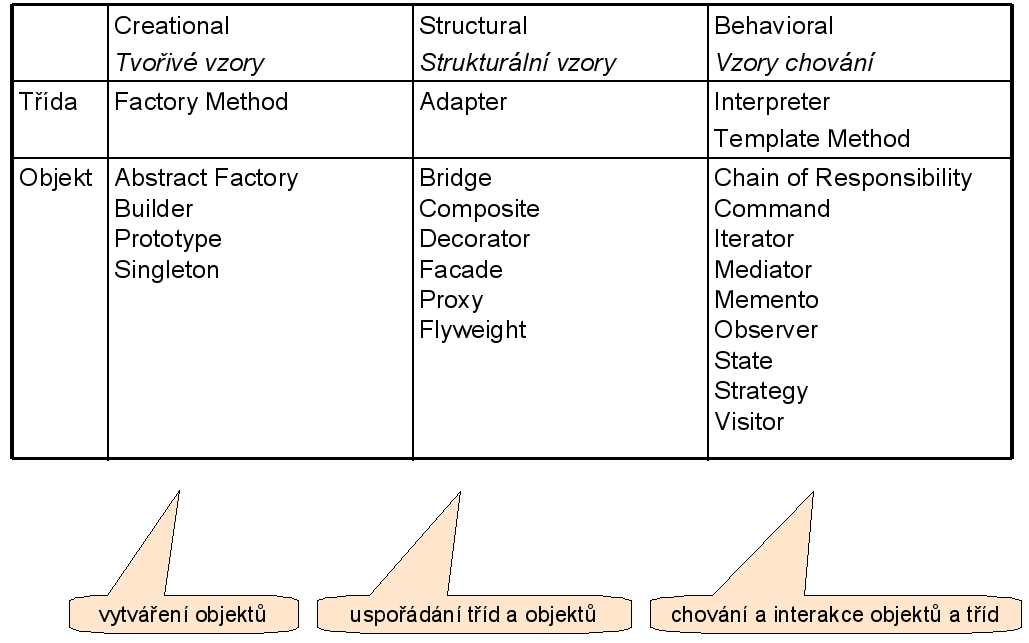
\includegraphics[width=12cm]{informatika/programovanie/obrazky/designpatterns.png}\end{center}
	
	Návrhové vzory je možno klasifikovat dle problémů které řeší. Príklady klasifikace vzorů podle řešených problémů:
	\begin{pitemize}
		\item \emph{Fundamental patterns}: ??? nevyhodíme to, je to jen na wiki a nepopsane
		\item \emph{Creation patterns}: vytváření objektů
		\item \emph{Structural patterns}: jak jsou třídy a objekty složený do větších struktur
		\item \emph{Behavioral patterns}: rozdělení funkčnosti a zodpovědnosti mezi objekty; komunikace mezi objekty; umožňuje zaměřit se při návrhu na propojení tříd, ne na běhové detaily
		\item \emph{Concurrency patterns} ??? tohle taky
	\end{pitemize}
}

\begin{priklady}
Creational patterns:
\begin{pitemize}
    \item Factory method (zajišťuje rozhodnutí o typu vytvářeného objektu při polymorfismu)
    \item Prototype (jak klonovat objekty)
    \item Singleton (jak omezit objekt jen na 1 instanci)
\end{pitemize}

Structural patterns:
\begin{pitemize}
    \item Adapter (konverze rozhraní objektů)
    \item Bridge (oddělení rozhraní a implementace třídy)
    \item Composite (jak složit více objektů do jednoho s jednotným přístupem)
    \item Proxy (jak zajistit přístup k jinému objektu přes můj objekt)
    \item Decorator (jak změnit vlastnosti třídy nebo zajistit rozšířenou funkčnost bez odděďování)
\end{pitemize}

Behavioral patterns:
\begin{pitemize}
    \item Chain of responsibility (jak určit kdo vykoná akci, když z venku přijde požadavek)
    \item Command (odstínění klienta od zpracování požadavku -- klient neurčuje kdy a jak se to provede)
    \item Iterator (projití prvků pole bez znalosti jejich implementace)
    \item Visitor (navštívení všech objektů nějaké struktury a práce s nimi, aby všechny nemusely implementovat stejné metody (a měnit se při jejich změně))
    \item Template (jak mohou odvozené třídy ovlivňovat algoritmy bázové třídy)
\end{pitemize}
\end{priklady}


TODO: rozšíriť, doplniť, opraviť :-)


\end{document}
